\label{Chapter3}

\chapter{A tool for Ethereum analytics}
\section{Architecture of the tool}
In this section we will describe how this tool works. This tool is build for create a custom view of either the Ethereum blockchain or the Bitcoin blockchain. Since we do not use Bitcoin blockchain, we will describe only how the Ethereum part works. We said the the view is \textit{custom} because this tool allows the user to extract whatever he needs from the blockchain, such as:
\begin{itemize}
    \item Blocks information, e.g. block number, block hash;
    \item Transactions information, e.g. transaction hash, sender, receiver, created contract (if exists);
    \item Contract internal transactions information, e.g. transaction hash, sender, receiver, father transaction hash (the transaction that calls the defined contract)
\end{itemize}

The following image describes the tool's architecture:
\begin{center}
    \[
        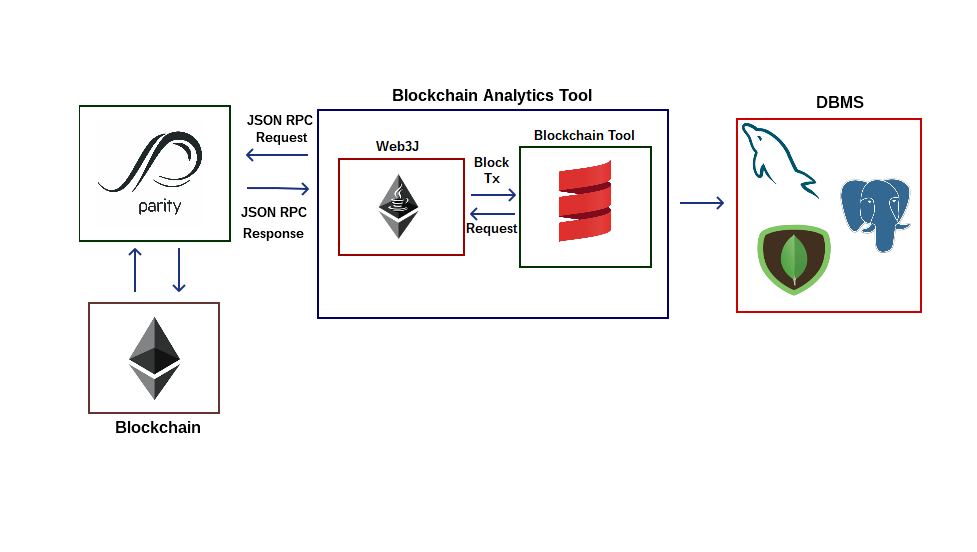
\includegraphics[
            trim=1cm 3cm 1cm 1cm,
            width=0.85\columnwidth,]{architecture.png}
    \]
\end{center}
As you can see, in order to retrieve blockchain data, our tool makes a request through Web3J (described in \ref{web3j}), which in turn makes a request directly to the Ethereum client, in our case Parity (described in \ref{parity}). This requests are made using the JSON-RPC protocol (described in \ref{jsonrpc}). 

When Parity returns the wanted result, Web3J serialize it into a collection of objects, then returns them to our tool. Since these classes do not contains all information, we decided to wrap them in another classes, retrieving all missing information, i.e. contract internal trasactions.

In the next subsections, we briefly describe how Parity, Web3J and JSON RPC work. Then, in the next sections, we show some view examples, using \textit{MongoDB} as DBMS.

\subsection{Parity}
\label{parity}
\href{https://www.parity.io/}{Parity} \cite{authors2017ethereum} is an Ethereum client, written from the ground-up for correctness-verifiability, modularisation, low-footprint and high-performance. \newline
To this end it utilises the Rust language, a hybrid imperative/OO/functional language with an emphasis on efficiency. 
\newline
Parity comes with an extensive, in-built Ethereum Wallet and DApp environment. It includes:
\begin{itemize}
    \item Account, address-book and multi-sig management.
    \item Key creation, importing and exporting.
    \item Web3 Ðapp browser.
    \item Hardware and electronic cold-wallet support.
    \item Name registry support.
    \item Contract development, deployment and interaction environment.
\end{itemize}

\subsection{Web3J}
\label{web3j}
\href{https://web3j.io/}{Web3J} is a highly modular, reactive, type safe Java and Android library for working with Smart Contracts and integrating with clients (nodes) on the Ethereum network. This allows to work with the Ethereum blockchain, without the additional overhead of having to write an integration code for the platform.

Web3J is capable to connect to a local blockchain, downloaded using Parity, \href{https://github.com/ethereum/go-ethereum/wiki/geth}{Geth} or another Ethereum client, or a remote one, like \href{https://infura.io}{Infura}.
In order to retrieve blockchain data, Web3J uses a protocol called JSON-RPC, which will be described in section \ref{jsonrpc}. 

\subsection{JSON-RPC}
\label{jsonrpc}
JSON-RPC \cite{json2012json} is a remote procedure call protocol encoded in JSON. It is a very simple protocol (and very similar to XML-RPC), defining only a few data types and commands. JSON-RPC allows for notifications (data sent to the server that does not require a response) and for multiple calls to be sent to the server which may be answered out of order.

JSON-RPC works by sending a request to a server implementing this protocol. The client in that case is typically software intending to call a single method of a remote system. Multiple input parameters can be passed to the remote method as an array or object, whereas the method itself can return multiple output data as well. (This depends on the implemented version).

All transfer types are single objects, serialized using JSON. A request is a call to a specific method provided by a remote system. It must contain three certain properties:
\begin{itemize}
    \item \textit{Method}: A String with the name of the method to be invoked;
    \item \textit{Params}: An Object or Array of values to be passed as parameters to the defined method;
    \item \textit{Id}: A value of any type used to match the response with the request that it is replying to.
\end{itemize}

The receiver of the request must reply with a valid response to all received requests. A response must contain the following properties:
\begin{itemize}
    \item \textit{Result}: The data returned by the invoked method. If an error occurred while invoking the method, this value must be null;
    \item \textit{Error}: A specified error code if there was an error invoking the method, otherwise null;
    \item \textit{Id}: The id of the request it is responding to.
\end{itemize}
Since there are situations where no response is needed or even desired, notifications were introduced. A notification is similar to a request except for the id, which is not needed because no response will be returned. In this case the id property should be omitted (Version 2.0) or be null (Version 1.0).
\subsubsection{Examples}
In this subsection, we will show one example of \textit{Request and Response} and one of \textit{Notification} using JSON-RPC version 2.0.
\newline
Request and response:
\begin{lstlisting}[language=json]
Request
{
    "jsonrpc": "2.0", 
    "method": "subtract", 
    "params": {
                "minuend": 42, 
                "subtrahend": 23
              },
    "id": 3
}
Response 
{
    "jsonrpc": "2.0", 
    "result": 19, 
    "id": 3
}
\end{lstlisting}
Notification, with no response
\begin{lstlisting}[language=json]
{
    "jsonrpc": "2.0",
    "method": "update",
    "params": [1,2,3,4,5]
}
\end{lstlisting}
\section{Case study: a basic view of the blockchain}
This view contains data about all transactions (and, contract internal transactions) that has been done inside Ethereum blockchain. The fields in this view are the following:
\begin{itemize}
    \item \textit{\textbf{txHash}}: transaction hash;
    \item \textit{\textbf{blockHeight}}: block number of the block that contains this transaction;
    \item \textit{\textbf{txIndex}}: transaction progressive number inside its block;
    \item \textit{\textbf{date}}: the date when block is mined;
    \item \textit{\textbf{from}}: transaction sender (the address of who is transferring money or creating a contract);
    \item \textit{\textbf{to}}: transaction receiver (the address of who is receiving money, this field is empty if this transaction creates a contract);
    \item \textit{\textbf{value}}: how much (in ETH) is transferred;
    \item \textit{\textbf{creates}}: the address of the newly created contract (empty if this transaction does not create a contract);
    \item \textit{\textbf{internalTransactions}}: contains all the internal transactions generated by this transaction, it's a list of objects containing the following fields:
        \subitem \textit{\textbf{parentTxHash}}: hash of the father transaction (the transaction that generates this one);
        \subitem \textit{\textbf{txType}}: internal transaction type (call, suicide, create);
        \subitem \textit{\textbf{from}}: internal transaction sender;
        \subitem \textit{\textbf{to}}: internal transaction receiver;
        \subitem \textit{\textbf{value}}: how much (in ETH) in transferred.
\end{itemize}
\subsection{Querying view in MongoDB}
\subsubsection{Ethereum per day}
This query calculates the total amount of Ether transacted and its mean per day.
\begin{center}
\begin{varwidth}{\linewidth}
\begin{verbatim}
db.myBlockchain.aggregate([
   { $group : {
       _id: {
           year : { $year : "$date" },
           month : { $month : "$date" },
           day : { $dayOfMonth : "$date" },
       },
       sumValues: { $sum: "$value"},
       avgValues: { $avg: "$value"}
   }},
   { $sort : { avgValues : 1, sumValues: 1}}
]);
\end{verbatim}
\end{varwidth}
\end{center}
\subsubsection{Contract creation}
This query search all transactions that create a smart contract. It returns only the created smart contract address. 
\begin{center}
\begin{varwidth}{\linewidth}
\begin{verbatim}
db.myBlockchain.find({
   creates: {$ne: ""}
},{
   _id: 0, creates: 1
});

\end{verbatim}
\end{varwidth}
\end{center}
\section{Case study: Exchange rates}
This view contains data about all transactions, combined with the Ethereum conversion price in USD in that specific day. 
The fields in this view are the following:
\begin{itemize}
    \item \textit{\textbf{txHash}}: transaction hash;
    \item \textit{\textbf{blockHeight}}: block number of the block that contains this transaction;
    \item \textit{\textbf{txIndex}}: transaction progressive number inside its block;
    \item \textit{\textbf{date}}: the date when block is mined;
    \item \textit{\textbf{from}}: transaction sender (the address of who is transferring money or creating a contract);
    \item \textit{\textbf{to}}: transaction receiver (the address of who is receiving money, this field is empty if this transaction creates a contract);
    \item \textit{\textbf{value}}: how much (in ETH) is transferred;
    \item \textit{\textbf{creates}}: the address of the newly created contract (empty if this transaction does not create a contract);
    \item \textit{\textbf{rate}}: Ethereum-USD conversion price.
\end{itemize}
\section{Case study: Levenshtein Distance between contract}
In information theory, Linguistics and computer science, the Levenshtein distance is a string metric for measuring the difference between two sequences.
In order to calculate Levenshtein distance between contracs EVM, first of all we create a view in MongoDB or SQL that contains only useful information retrieved from blockchain.
The useful fields are only two:
\begin{itemize}
    \item \textit{\textbf{contractAddress}}: The contract address inside blockchain (to uniquely identify a contract inside view);
    \item \textit{\textbf{contractCode}}: The contract EVM code
\end{itemize}
The distance calculation is done using this formula:
\begin{center}
$\operatorname{lev}_{a,b}(i,j) = 
\begin{cases}
  \max(i,j) & \text{ if} \min(i,j)=0, \\
  \min \begin{cases}
      \operatorname{lev}_{a,b}(i-1,j) + 1 \\
      \operatorname{lev}_{a,b}(i,j-1) + 1 \\
      \operatorname{lev}_{a,b}(i-1,j-1) + 1_{(a_i \neq b_j)}
   \end{cases} & \text{ otherwise.}
\end{cases}
$
\end{center}


\section{Implementation}
In this section we will explain in details the implementation of the tool, built to retrieve blockchain data and other external data and combine them. \newline
This tool is written in Scala Programming Language and built with Scala Build Tool (SBT). \newline
Scala has been chosen because, since it's compiled in bytecode that runs on Java Virtual Machine (JVM), it can be combined with Java external libraries without any problem. \newline
Thanks to this property, it was possible to use Web3J library to retrieve blockchain data. It is a Java and Android library for working with Smart Contracts and integrating with clients (nodes) on the Ethereum network. \newline
Web3J is the Java version of a Web3 (a Javascript library), which has be explained in \ref{web3j}. In the following paragraph, we explain the created classes.